\documentclass[10pt,a4paper]{article}
\usepackage[utf8]{inputenc}
\usepackage{amsmath}
\usepackage{amsfonts}
\usepackage{siunitx}
\usepackage[european]{circuitikz}
\usepackage{geometry}
\newgeometry{tmargin=2cm, bmargin=2cm, lmargin=2cm, rmargin=2cm}
\usepackage{amssymb}
\usepackage{polski}
\usepackage{graphicx}
\author{\textbf{T. Fąs}}
\title{\textbf{PRAWO OHMA I KIRCHHOFFA}}
\begin{document}
\maketitle

\begin{center}
\textbf{\subsection*{STRESZCZENIE}}
\end{center}
Celem doświadczenia było sprawdzenie słuszności prawa Ohma i praw Kirchhoffa oraz wyznaczenie oporu wewnętrznego i siły elektromotorycznej baterii. Do wyznaczenia tych wielkości zastosowano wyżej wymienione prawa. Przeprowadzone pomiary wykazały zgodność z prawami Ohma i Kirchhoffa, z drobnymi zastrzeżeniami w przypadku pierwszego prawa Kirchhoffa. Wyznaczona wartość oporu własnego to $ r=0,5$ $ \Omega$, a wartość SEM to $ \mathcal{E}=1,489 $ V.
\begin{center}
\textbf{\subsection*{WSTĘP}}
\end{center}
Prawo Ohma głosi, że natężenie prądu $I$ płynącego przez przewodnik jest wprost proporcjonalne do przyłożonego napięcia $U$; lub inaczej: stosunek napięcia do natężenia prądu jest stały i równy oporowi $R$ przewodnika:
\begin{equation}
R=\dfrac{U}{I} \quad  \cite{hrw1}.
\label{r1}
\end{equation}
Aby wyznaczyć opór trzeba zmierzyć wartości napięcia na oporze oraz przepływającego przezeń prądu. Otrzymane wartości oporu można wtedy porównać ze zmierzoną niezależnie wartością oporu. Ich zgodność będzie potwierdzeniem słuszności prawa Ohma.

Pierwsze prawo Kirchhoffa głosi, że sumy natężeń prądów wpływających i wypływających z węzła sieci są sobie równe. \cite{hrw2} Znaczy to, że jeśli przewód rozdziela się na trzy inne, to suma natężeń w tych trzech przewodach musi być równa natężeniu w pierwotnym przewodzie. W takim wypadku należy zmierzyć wartości natężeń prądów w poszczególnych gałęziach sieci i korzystając z prawa Kirchhoffa przyrównać sumy natężeń prądów wpływających i wypływających. Ich równość będzie potwierdzeniem prawa Kirchhoffa. 

Z prawa Ohma i pierwszego prawa Kirchhoffa wynikają również reguły sumowania oporników podłączonych szeregowo lub równolegle. Dla $n$ oporników podłączonych równolegle wzór na sumę oporów $R_{z}$ ma postać:
\begin{equation}
\dfrac{1}{R_{z}}=\sum_{j=1}^{i}\dfrac{1}{R_{j}},
\label{r2}
\end{equation}
gdzie $R_{j}$ są kolejnymi opornikami podłączonymi równolegle.
Drugie prawo Kirchhoffa głosi, że suma wzrostów i spadków napięć w obwodzie zamkniętym jest równa zeru \cite{hrw3}.
Zmierzenie wartości oporu wewnętrznego r baterii o SEM$=\mathcal{E}$ wymaga skorzystania z praw Ohma i obu praw Kirchhoffa. Mierząc natężenie prądu w obwodzie z baterią i opornikiem oraz napięcie na baterii otrzymamy wartości $I$ oraz $U$. Z prawa Ohma oraz II prawa Kirchhoffa wiadomo, że:
\begin{eqnarray}
U=IR \\
\label{r3}
\mathcal{E}-Ir-IR=0
\label{r4}
\end{eqnarray}
Rozwiązując ten układ Równań (\ref{r3}) i (\ref{r4}) ze względu na $U$ otrzymano zależność:
\begin{equation}
U(I)=-rI+\mathcal{E}
\label{r5}
\end{equation}
Jest to równanie prostej $y=ax+b$ o współczynnikach $a=-r$ i $b=\mathcal{E}$. Aby poznać wartości oporu wewnętrznego baterii oraz jej SEM wystarczy poznać wartości współczynników prostej najlepszego dopasowania.

Innym celem tego ćwiczenia było dopasowanie krzywej Gaussa do histogramu gęstości 216 okresów wahadła. Modelowa gęstość rozkładu okresów T jest dana wzorem:
\begin{equation}
G(T;\mu,\sigma)=\dfrac{1}{\sqrt{2\pi}\sigma}\exp \left(-\dfrac{(T-\mu)^2}{2\sigma^2}\right),
\label{r6}
\end{equation}
gdzie $\sigma$ jest odchyleniem standardowym pomiarów, a $\mu$ jest wartością oczekiwaną pomiaru \cite{g1}.
Aby znaleźć liczbę oczekiwanych pomiarów $N_{k}$ z serii $N$ pomiarów w danym przedziale, należy posłużyć się wzorem:
\begin{equation}
N_{k}=N\int_{T_{k}}^{T_{k}+\Delta}G(T;\mu,\sigma)dT,
\label{r7}
\end{equation}
gdzie $T_{k}$ jest początkiem przedziału, a $\Delta$ jego szerokością.
Porównanie wartości otrzymanych na drodze eksperymentu z wartościami teoretycznymi pozwoli na ocenę tego, czy dane przeczą hipotezie, czy też są z nią niesprzeczne. W tym przypadku posłużono się tylko wizualną oceną dopasowania krzywej do histogramu. W przypadku oceniania danych otrzymanych dla prawa Ohma i Kirchhoffa posłużono się testem $3\sigma$. Polega on na sprawdzeniu, czy różnica pomiędzy wartością oczekiwaną, a otrzymaną nie przekracza trzykrotności odchylenia standardowego.
\begin{center}
\textbf{\subsection*{UKŁAD DOŚWIADCZALNY}}
\end{center}
Do wykonywania pomiarów wykorzystano miernik Brymen 805 oraz miernik CHY 38. Niepewności pomiaru miernika Brymen obliczono na podstawie instrukcji dołączonej przez producenta \cite{b1}. Wykorzystano dodatkowo oporniki o wartościach oporu powyżej i poniżej $1$ k$\Omega$. Jako zasilanie wykorzystano zasilacz generujący prąd o stałym napięciu, które w czasie pomiarów regulowano. Rysunek \ref{p1} przedstawia schemat płytki drukowanej, którą wykorzystano do testowania praw Ohma i Kirchhoffa. Do zacisków E$-$ i E$+$ podłączono zasilanie. Do zacisków R1, R2 i R3 podłączano oporniki. Reszta zacisków służyła jako przełączniki, które były otwarte lub zamknięte, w zależności od potrzeb.
\begin{figure}[h]
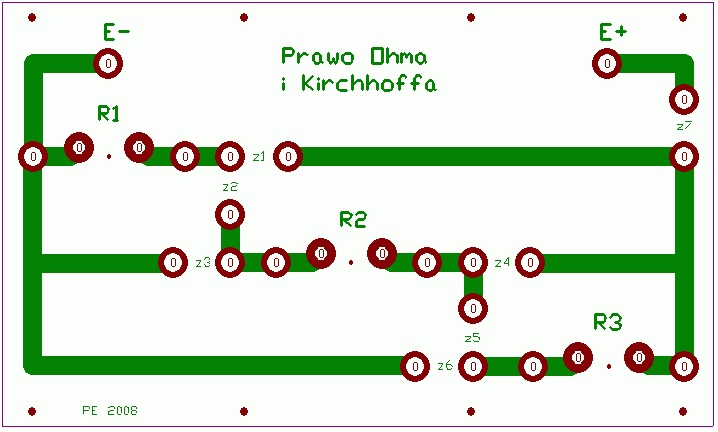
\includegraphics[width=8cm]{UKLAD} 
\centering
\caption{Układ do sprawdzenia praw Ohma i Kirchhoffa}
\label{p1}
\end{figure}

Na potrzeby sprawdzenia prawa Ohma do zacisków R1 podłączono kiloomowy opornik, a zaciski z1 i z7 zamknięto. Do zacisków E$-$ i E$+$ podłączono zasilanie, z kolei do zacisków po lewej i prawej stronie R1 podłączono miernik CHY w charakterze woltomierza. Zacisk z1 zamknięto miernikiem Brymen w charakterze amperomierza. Na generatorze regulowano napięcie od 0 do 20 V, które następnie odczytywano na mierniku CHY, z kolei natężenie prądu odczytywano z miernika Brymen. 

Dla drugiego prawa Kirchhoffa zamknięto zaciski z2, z5 i z7, a do zacisków R1, R2 i R3 podłączono kiloomowe oporniki. Podłączenie zacisków w taki sposób tworzy szeregowe połączenie oporników. Miernik Brymen, jako woltomierz podłączano do zacisków po lewej i prawej stronie kolejno R1, R2 i R3, a także, aby zmierzyć napięcie, jak i opór na całym obwodzie, do zacisków po lewej stronie R1 i prawej stronie R3.

Na potrzeby testu pierwszego prawa Kirchhoffa do zacisków R1, R2 i R3 podłączono kiloomowe oporniki, a zaciski z1, z3, z4, z6 i z7 zamknięto.  Podłączenie zacisków w taki sposób tworzy równoległe połączenie oporników. Zaciski zamykano miernikiem Brymen, jako amperomierzem, którego wskazywania odczytywano, a następnie zmieniano jego pozycję. Opór całkowity zmierzono tym samym miernikiem podłączonym do zacisków po lewej stronie R1 i prawej stronie R3.

Do znalezienia oporu wewnętrznego baterii wykorzystano układ przedstawiony na Rysunku \ref{p2}.

\begin{figure}[h!]
 
\tikzset{component/.style={draw,thick,circle,fill=white,minimum size =0.75cm,inner sep=0pt}}
\begin{circuitikz} \draw
(0,0) to node[component]{V} (0,4) --(2,4)
     to [ battery1=$\mathcal{E}$, *-,] (2,2)
     to [R, -*, l={r}] (2,0) --(0,0) 
     to [short,-o] (5,0) --(5.5,0.3)
     (5.5,0.3) to [open,-o] (5.5,0) --(6,0)
     to [R, l=${R_{z}}$] (6,4)
     to node[component]{A} (4,4) --(2,4)     
;
\end{circuitikz}
\centering
 \caption{Układ wykorzystany do znalezienia oporu wewnętrznego baterii}
 \label{p2}
\end{figure}
Strzałka oznacza tu kierunek przepływu prądu, $\mathcal{E}$ oznacza SEM baterii, $r$ jej opór wewnętrzny, a $R_{z}$ to opornik podłączony do układu. Jako $R_{z}$ podłączano różne oporniki o oporności poniżej $1$ k$\Omega$. W roli amperomierza i woltomierza posłużono się miernikami Brymen. 

\begin{center}
\textbf{\subsection*{WYNIKI POMIARÓW}}
\end{center}
Testując prawo Ohma zmierzono rezystancję opornika $R_{1}=10,84$ k$\Omega$. Następnie wykonano serię 10 pomiarów napięcia i natężenia w obwodzie z podłączonym opornikiem $R_{1}$. Wyniki zaprezentowano w Tabeli \ref{t1}.
\begin{center}
 \begin{table}[h!]
 \centering
 \caption{Prawo Ohma: wyniki pomiarów }
 \label{t1}
 \begin{tabular}{|c|c|c|c|c|c|c|c|c|c|c|}
 \hline
 Napięcie $U$ [V] &1,99 & 4,05&6,12 & 8,07& 10,00&12,11&14,05&15,98&17,19&18,86 \\
 \hline
 Natężenie $I$ [mA]& 0,18 &0,37&0,56&0,74&0,92&1,11&1,3&1,48&1,59&1,74 \\
 \hline
 \end{tabular}
 \end{table}
 \end{center}
 W dalszej części dodano dwa kolejne oporniki o rezystancji $R_{2}=8,22$ k$\Omega$ i $R_{3}=3,260$ k$\Omega$. Wynik pomiaru oporu całkowitego wszystkich trzech oporników wynosi $R_{c}=22,32$ k$\Omega$. Następnie wykonano pomiary napięcia na opornikach i na całości obwodu. Wyniki zaprezentowano w Tabeli \ref{t2}. 
 \begin{center}
 \begin{table}[h!]
 \centering
 \caption{Drugie prawo Kirchhoffa: wyniki pomiarów }
 \label{t2}
 \begin{tabular}{|c|c|c|c|c|c|c|c|c|c|c|}
 \hline
 Opornik&$R_{1}$& $R_{2}$&$R_{3}$ &Całość \\
 \hline
 Napięcie $U$ [V]& 2,909 &2,205&0,874&5,99 \\
 \hline 
 \end{tabular}
 \end{table}
 \end{center}
  Wyniki pomiarów dla testu pierwszego prawa Kirchhoffa przedstawia Tabela \ref{t3}. Poprzez oznaczenia oporników oznaczono gałęzie, w których dokonano pomiarów natężenia; dana gałąź zawierała tylko jeden opornik. 
 \begin{center}
 \begin{table}[h!]
 \centering
 \caption{Pierwsze prawo Kirchhoffa: wyniki pomiarów }
 \label{t3}
 \begin{tabular}{|c|c|c|c|c|c|c|c|c|c|c|}
 \hline
 Opornik&$R_{1}$& $R_{2}$&$R_{3}$ &Całość \\
 \hline
 Natężenie $I$ [$\mu$A]& 550 &724&1790&2978 \\
 \hline 
 \end{tabular}
 \end{table}
 \end{center}
 Przy czym zmierzona wartość oporu całkowitego obwodu wynosi $R_{z}=1,919$ k$\Omega$.
 
 Ostatnie pomiary dotyczyły pomiarów natężenia i napięcia w obwodzie związanym z baterią i jej oporem wewnętrznym. Obwód skonstruowany tak, jak na Rysunku \ref{p2} zamykano na czas pomiarów, które dokonywano możliwie szybko, aby nie wyczerpać baterii. Wykonano pięć pomiarów, przy pięciu różnych opornikach $R$ oraz jeden pomiar bez żadnego opornika. Wyniki zaprezentowano w Tabeli \ref{t4}. 
  \begin{center}
 \begin{table}[h!]
 \centering
 \caption{Bateria: wyniki pomiarów }
 \label{t4}
 \begin{tabular}{|c|c|c|c|c|c|c|c|c|c|c|}
 \hline
 Napięcie $U$ [V]&1,495& 1,485&1,481 &1,479& 1,474&1,466 \\
 \hline
 Natężenie $I$ [mA]& 0 &7,69&12,88&20,06&29,78&45,8 \\
 \hline 
 \end{tabular}
 \end{table}
 \end{center}
\begin{center}
\textbf{\subsection*{ANALIZA DANYCH}}
\end{center} 
Na początku zajęto się kwestią histogramu i krzywej Gaussa dla 216 okresów drgań wahadła. Dane zostały dostarczone przez prowadzących ćwiczenia. Średni okres $\bar{T}$ wynosi $3,4408$ s, a odchylenie standardowe $\sigma=0,0456$ s. Na ich podstawie stworzono histogram gęstości okresów oraz dopasowano do niego krzywą Gaussa. Sam wykres znajduje się na Rysunku 3. Dane, które posłużyły do jego skonstruowania są zaprezentowane w Tabeli \ref{t5}. Wartości gęstości $G$ oraz $N_{k}$ obliczono na podstawie wzorów (\ref{r6}) i (\ref{r7}), aczkolwiek Równanie (\ref{r7}) uproszczono do postaci:
\begin{equation}
\label{r8}
N_{k}\approx N_{k}^{'}=NG\left(T_{k};\bar{T},s_{T}\right)\Delta
\end{equation}
Celem dokładniejszego wyznaczenia całki z Równania (\ref{r7}) wprowadzono nową zmienną:
\begin{equation*}
 z=\dfrac{T-\mu}{\sigma}
 \end{equation*} 
 i za jej pomocą wyznaczono dokładniejszą wartość $N_{k}$:
 \begin{equation}
 \label{r9}
 N_{k}=N\left(F(z_{k+1}-F(z_{k})\right),
 \end{equation} 
 gdzie 
 \begin{equation*}
 z_{k}=\dfrac{T_{k}-\mu}{\sigma}, \quad  z_{k+1}=\dfrac{T_{k+1}+\Delta-\mu}{\sigma}, \quad F(z)=\dfrac{1}{\sqrt{2\pi}}\int_{-\infty}^{z}\exp{-\dfrac{x^2}{2}}dx.
 \end{equation*} 
  
  Ostatecznie, przy obliczeniach skorzystano z Równania (\ref{r6}), Równania (\ref{r8}) i  Równania (\ref{r9}).
  \begin{center}
 \begin{table}[h!]
 \centering
 \caption{Wyniki pomiarów i obliczeń dla 216 okresów drgań wahadła}
 \label{t5}
 \begin{tabular}{|c|c|c|c|c|c|c|c|c|c|c|}
 \hline
 Krawędź dolna $T_{k}$ [s]&3,25&3,30&3,35&3,40&3,45&3,50&3,55&3,60&$-$ \\
 \hline
 Krawędź górna $T_{k}+\Delta$ [s]&3,30&3,35&3,40&3,45&3,50&3,55&3,60&3,65&$-$ \\
 \hline 
 Środek przedziału $T_{k}$ [s]& 3,275&3,325&3,3,375&3,425&3,475&3,525&3,575&3,625&Suma$=$\\
 \hline
 Liczba $n_{k}$ danych&0&5&43&91&63&13&1&0&$N=216$\\
 \hline
 Gęstość eksperymentalna [s$^-1$]& 0,00&0,46&3,98&8,43&5,83&1,20&0,09&0,00&$-$\\
 \hline
 Gęstość $G\left(T_{k};\bar{T},s_{T}\right)$&0,01&0,35&3,09&8,24&6,60&1,59&0,12&0,00&$-$\\
 \hline
 $N_{k}^{'}$&0,127&3,758&33,360&88,981&71,322&17,179&1,243&0,027&215,971\\
 \hline
 $N_{k}$&0,215&4,799&35,043&85,208&69,758&19,178&1,744&0,051&215,996\\
 \hline
 \end{tabular}
 \end{table}
 \end{center}
 Przyglądając się Rysunkowi 3 oraz porównując wartości $n_{k}$ i $N_{k}$ można wyciągnąć wniosek, iż dane pokrywają się z krzywą Gaussa. Pozwala to na założenie, że wartością prawdziwą okresu jest wartość średnia, a niepewności są pochodzenia statystycznego. Krzywa Gaussa nie pokrywa się jednak idealnie z histogramem, wynika to z szerokości jego przedziałów. Gdyby wybrać mniejszą szerokość $\Delta$ przedziałów coraz bardziej zbliżałby się do krzywej.
 
 Testowanie prawa Ohma: z danych z Tabeli \ref{t1} utworzono wykres przedstawiony na Rysunku 4. Zgodnie z Równaniem (\ref{r1}) zależność $U(I)$ jest zależnością liniową o współczynniki kierunkowym równym oporowi. Współczynnik kierunkowy obliczono dla punktów $U=4,05$ V, $I=0,37$ mA oraz $U=10,00$ V i $I=0,92$ mA. Wynika stąd, iż prosta jest dana równaniem: $U(I)=10,82I+0,0466$, gdzie $a=10,82\dfrac{V}{mA}=10,82$ k$\Omega$ jest bliski zmierzonemu oporowi $R_{1}=10,84$ k$\Omega$, z kolei $b=0,0466$ V jest bliskie zeru. Otrzymane wyniki stanowią potwierdzenie prawa Ohma. 
 

 Dopuszczalny graniczny błąd wskazania na danym zakresie pomiarowym miernika wyznaczono na podstawie wzoru:
\begin{equation}
\label{r10}
\Delta_{p}=wx+nc,
\end{equation}
gdzie poszczególne symbole oznaczają: x – wynik pomiaru, w – dokładność wskazanej wartości x wyrażona w procentach, nc – dokładność cyfrowa określana jako liczba n najmniej znaczących jednostek c odczytu. Wielkości w, n oraz c odczytano z instrukcji miernika dołączonej przez producenta. Aby wyznaczyć niepewności pomiarów dla testu pierwszego i drugiego prawa Kirchhoffa posłużono się metodą propagacji małych błędów, daną wzorem:
 \begin{equation}
 \label{r11}
 u_{f}^2=\sum_{i=1}^n \left( \dfrac{\partial f}{\partial x_{i}}u_{i}\right) ^2,
 \end{equation}
 gdzie $u_{f}$ jest niepewnością szukanej wielkości zależnej od $x_{i}$, a $u_{i}$ jest niepewnością $x_{i}$ daną wzorem:
 \begin{equation}
  u_{i}^2=\dfrac{\Delta_{p}^2}{3} \quad \cite{tay3}.
  \end{equation} 
 Na podstawie tych wzorów stworzono Tabelę \ref{t6}.
 
  \begin{center}
 \begin{table}[h!]
 \centering
 \caption{Tabela wyników i niepewności pomiarów}
 \label{t6}
 \begin{tabular}{|c|c|c|c|c|c|c|c|c|c|c|}
 \hline
 Opornik&$R_{1}$& $R_{2}$&$R_{3}$ &Całość \\
 \hline
 Napięcie $U$ [V]& 2,909 &2,205&0,874&5,99 \\
 \hline 
 Składowa w niepewności&0,005&0,005&0,005&0,005\\
 \hline
 Składowa nc&0,003&0,003&0,003&0,03\\
 \hline
 Dopuszczalny błąd $\Delta_{V_{i}}$ [V]&0,01755&0,01403&0,00737&0,05995\\
 \hline
 Niepewność $u_{i}$ napięcia [V] &0,01013&0,00810&0,00426&0,03461\\
 \hline
 \end{tabular}
 \end{table}
 \end{center}
Na potrzeby testu drugiego prawa Kirchhoffa obliczono sumę wszystkich napięć $U_{S}$, moduł różnicy $U_{r}$ sumy i całego zmierzonego napięcia $U_{C}$ oraz ich niepewności. Niepewności te, wyznaczone z Równania (\ref{r11}), dane są wzorami:
 \begin{eqnarray}
u_{U_{S}}^{2}=u_{U_{R1}}^{2}+u_{U_{R2}}^{2}+u_{U_{R3}}^{2} \\
\label{r12}
u_{U_{r}}^2=u_{U_{S}}^2+u_{U_{C}}^2
\label{r13}
\end{eqnarray}
Obliczone wartości wstawiono do Tabeli \ref{t7}.
\begin{center}
\begin{table}[h!]
 \centering
 \caption{Tabela wyników i niepewności pomiarów}
 \label{t7}
 \begin{tabular}{|c|c|c|c|c|c|c|c|c|c|c|}
 \hline
 $U_{S}$ [V]&$U_{C}$ [V]& $U_{r}$ [V]&$u_{U_{S}}$ [V] &$u_{U_{r}}$ [V] \\
 \hline
 5,988&5,990&0,00200&0,01365&0,03721\\
 \hline
 \end{tabular}
 \end{table}
 \end{center}
Aby przejść test $3\sigma$ stosunek $U_{r}/u_{U_{r}}$ musi być mniejszy od $3$. Obliczona wartość tego stosunku wynosi 0,05375, która jest znacznie mniejsza od 3. Pozwala to stwierdzić iż otrzymane wyniki nie są sprzeczne z drugim prawem Kirchhoffa.

Analogiczne obliczenia wykonano dla pierwszego prawa Kirchhoffa, czyli Tabeli \ref{t3}. Wyniki obliczeń zapisano w Tabeli \ref{t8}.
 \begin{center}
 \begin{table}[h!]
 \centering
 \caption{Tabela wyników i niepewności pomiarów}
 \label{t8}
 \begin{tabular}{|c|c|c|c|c|c|c|c|c|c|c|}
 \hline
 Opornik&$R_{1}$& $R_{2}$&$R_{3}$ &Całość \\
 \hline
Natężenie I [$\mu$A]&550 &724&1790&2978 \\
 \hline 
 Składowa w niepewności&0,012&0,012&0,012&0,012\\
 \hline
 Składowa nc&3&3&3&3\\
 \hline
 Dopuszczalny błąd $\Delta_{I_{i}}$ [$\mu$A]&9,6000&11,6880&24,4800&38,7360\\
 \hline
 Niepewność $u_{i}$ natężenia I [$\mu$A] &5,54256&6,74807&14,13353&23,36424\\
 \hline
 \end{tabular}
 \end{table}
 \end{center}
Wzory (\ref{r12}) i (\ref{r13}), jak i cała procedura stosują się również do natężeń. Tak więć można stworzyć analogiczną tabelę z wynikami oraz wykonać test $3\sigma$.
\begin{center}
\begin{table}[h!]
 \centering
 \caption{Tabela wyników i niepewności pomiarów}
 \label{t9}
 \begin{tabular}{|c|c|c|c|c|c|c|c|c|c|c|}
 \hline
 $I_{S}$ [mA]&$I_{C}$ [mA]& $I_{r}$ [mA]&$u_{I_{S}}$ [mA] &$u_{I_{r}}$ [mA]& $I_{r}/u_{I_{r}}$ \\
 \hline
 3,064&2,978&0,086&0,01661&0,02786&3,08688\\
 \hline
 \end{tabular}
 \end{table}
 \end{center}
 Jak widać w Tabeli \ref{t9}, wykonane pomiary zdają się przeczyć pierwszemu prawu Kirchhoffa. Trzeba jednak wziąć pod uwagę, że mogły wystąpić pewne niedokładności samego obwodu w postaci np. poluzowanego zacisku czy też drobne fluktuacje natężenia   generowanego przez zasilacz. Nie brano pod uwagę niedokładności obwodu czy też zasilacza, dlatego też wyniki mogą zdawać się przeczyć prawu Kirchhoffa, choć błąd znajduje się po stronie eksperymentatora. Wziąwszy pod uwagę niewielkie odstępstwo od wartości 3 obliczonego stosunku można założyć, że wyniki nie odbiegają aż tak bardzo od oczekiwanej wartości, ale granica jest ścisła, więc test $3\sigma$ dla pierwszego prawa Kirchhoffa nie został zaliczony.  
 
Aby sprawdzić słuszność Równania (\ref{r2}) należy przeprowadzić analizę podobną do tej przeprowadzonej dla praw Kirchhoffa. Tabela \ref{t10} przedstawia wyniki obliczeń opartych na Równaniach (\ref{r10}) i (12) przeprowadzonych dla wartości oporów $R_{1}$, $R_{2}$ i $R_{3}$ oraz ich oporu zastępczego $R_{z}$.

 \begin{center}
 \begin{table}[h!]
 \centering
 \caption{Tabela wyników i niepewności pomiarów}
 \label{t10}
 \begin{tabular}{|c|c|c|c|c|c|c|c|c|c|c|}
 \hline
 Opornik&$R_{1}$& $R_{2}$&$R_{3}$ &$R_{z}$ \\
 \hline
Opór R [k$\Omega$]&10,84 &8,22&3,260&1,919 \\
 \hline 
 Składowa w niepewności&0,006&0,006&0,006&0,006\\
 \hline
 Składowa nc&0,04&0,04&0,004&0,004\\
 \hline
 Dopuszczalny błąd $\Delta_{R_{i}}$ [k$\Omega$]&0,10504&0,08932&0,02356&0,01551\\
 \hline
 Niepewność $u_{i}$ [k$\Omega$] &0,06064&0,05157&0,01360&0,00896\\
 \hline
 \end{tabular}
 \end{table}
 \end{center}
Sumę oporów $R_{S}$ obliczono, korzystając z Równania (\ref{r2}). Niepewność tej sumy dana jest wzorem:
\begin{equation}
 u_{Rz}^2=R_{z}^4\left(\dfrac{u_{R_{1}}^2}{R_{1}^4}+\dfrac{u_{R_{2}}^2}{R_{2}^4}+\dfrac{u_{R_{3}}^2}{R_{3}^4}\right)
 \end{equation} 
 Korzystając z Równania (2), Równania (15) oraz obliczają różnicę $R_{r}$ oporów wyliczonego i zmierzonego stworzono Tabelę \ref{t11}. Niepewność różnicy dana jest wzorem analogicznym do Równania (\ref{r13}).
 \begin{center}
\begin{table}[h!]
 \centering
 \caption{Tabela wyników i niepewności pomiarów}
 \label{t11}
 \begin{tabular}{|c|c|c|c|c|c|c|c|c|c|c|}
 \hline
 $R_{S}$ [k$\Omega$]&$R_{z}$ [k$\Omega$]& $R_{r}$ [k$\Omega$]&$u_{R_{S}}$ [k$\Omega$] &$u_{R_{r}}$ [k$\Omega$]& $R_{r}/u_{R_{r}}$ \\
 \hline
 1,92066&1,91900&0,00166&0,00582&0,01068&0,0,15559\\
 \hline
 \end{tabular}
 \end{table}
 \end{center}
Jak widać, test $3\sigma$ został zaliczony, otrzymane wyniki nie są sprzeczne z hipotezą. 

Korzystając z danych z Tabeli \ref{t4} wykonano wykres zależności $U(I)$ przedstawiony na Rysunku 5. Parametry prostej obliczono dla punktów $U=1,485$ V, $I=7,69$ mA oraz $U=1,466$ V i $I=45,8$ mA. Otrzymano wartości $a=-0,0005$ V/mA oraz $b=1,489$ V. Zgodnie z zależnością wyprowadzoną w Równaniu (\ref{r5}) opór wewnętrzny baterii jest równy 0,5 $\Omega$ a jej SEM jest równa 1,489 V. Otrzymana wartość oporu wewnętrznego jest typowa dla baterii tego typu. Wątpliwości budzi jednak otrzymana wartość SEM, która nie pokrywa się z wartością zmierzoną. Jednak w tym przypadku błąd znajduje się po stronie eksperymentatora. Wykonano dwie serie pomiarowa, ponieważ w pierwszej z nich miernik wskazywał błędne wartości natężenia. Dlatego też wykonano drugą serię pomiarową, jednak nie wykonano ponownie pomiaru napięcia na samej baterii, bez opornika. Dlatego też otrzymana wartość SEM jest niższa; wynika to z rozładowania baterii. Otrzymana wartość wskazuje SEM baterii przed drugą serią pomiarową i jest to wartość poprawna, biorąc pod uwagę jej rozładowanie i ignorując pierwotny pomiar napięcia bez opornika.

\begin{center}
\textbf{\subsection*{DYSKUSJA WYNIKÓW I WNIOSKI}}
\end{center} 
Prawie wszystkie przeprowadzone testy praw Ohma i Kirchhoffa wykazały słuszność tych praw, z wykluczeniem testu dla pierwszego prawa Kirchhoffa. Jedna zważywszy na niewielkie odchylenie od wartości $\sigma$ oraz wziąwszy pod uwagę niedokładności układu można stwierdzić, iż również i ten test nie jest sprzeczny z prawem Kirchhoffa. Aby móc mieć absolutną pewność należałoby przeprowadzić dodatkowe pomiary. 

W przypadku wyznaczania oporu wewnętrznego baterii oraz jej SEM również napotkano na problemy dotyczące wartości SEM baterii, jednak ten problem bez problemu rozwiązano, a zaprezentowana wartość SEM jest prawdziwa i zgodna z przewidywaniami. Jednak tak jak w przypadku prawa Kirchhoffa, całkowitą pewność można uzyskać dopiero po ponownym przeprowadzeniu pomiarów. 

Jednak pomimo tych wszystkich niepewności otrzymane wyniki były zgodne z przewidywaniami, nawet te budzące zastrzeżenia, ponieważ ich odchylenia od wartości oczekiwanych były niewielkie. Podsumowują, można powiedzieć, iż wszystkie otrzymane wyniki są zgodnie z przewidywaniami i nie są sprzeczne z prawem Ohma oraz prawami Kirchhoffa.

\begin{center}
\begin{thebibliography}{9}

\bibitem{hrw1}
 D. Halliday, R. Resnick, J. Walker,
  \emph{Podstawy Fizyki, Tom 3},
  PWN, Warszawa, 2003, s. 140.
  
  \bibitem{hrw2}
 D. Halliday, R. Resnick, J. Walker,
  \emph{Podstawy Fizyki, Tom 3},
  PWN, Warszawa, 2003, s. 165.
  
  \bibitem{hrw3}
 D. Halliday, R. Resnick, J. Walker,
  \emph{Podstawy Fizyki, Tom 3},
  PWN, Warszawa, 2003, s. 158.
  
  \bibitem{g1}
  N. W. Smirnow, I. W. Dunin-Barkowski,
  \emph{Kurs rachunku prawdopodobieństwa i statystyki matematycznej dla zastosowań technicznych},
  PWN, Warszawa, 1973, s. 151.
  
   \bibitem{b1}
  Praca zbiorowa,
  \emph{Multimetry cyfrowe BM805, BM806T, BM807},
  BRYMEN Technology Co., Taiwan, s. 20.
  
  \bibitem{tay3}
 J. R. Taylor,
 \emph{Wstęp do analizy błędu pomiarowego},
 PWN, Warszawa, 1995, s. 87.
  
  \end{thebibliography}
\end{center}
\end{document}